\documentclass[finals,table,dvipsnames]{beamer}
\usefonttheme{professionalfonts}

\usepackage[english]{babel}
\usepackage[utf8]{inputenc}
\usepackage[T1]{fontenc}
\usepackage{amsmath}
\usepackage{multicol}
\usepackage{graphicx}
\usepackage{hyperref}
\usepackage{float}
\usepackage{url}
\usepackage{wasysym}
\usepackage{xspace}
\usepackage{times}
\usepackage{booktabs}
\usepackage{xcolor}
\usepackage{marvosym}
\usepackage{tikz}
\usepackage{listings}
\usepackage{fancybox}
\usepackage{shadow}


\usetikzlibrary{arrows,shapes,backgrounds}
\tikzstyle{every picture}+=[remember picture]
\tikzstyle{na} = [baseline=-.5ex]

\DeclareGraphicsExtensions{.eps,.pdf,.JPG,.jpg,.jpeg,.png,.PNG}
\graphicspath{
{./figures/}
}
\definecolor{sdnblue}{HTML}{005baa}
\definecolor{sdngrey}{HTML}{646464}

\setbeamertemplate{navigation symbols}{}
\setbeamercolor{title}{fg=sdnblue}
\setbeamertemplate{footline}[frame number]
%\setbeamercolor{background canvas}{bg=black!95}
%\setbeamercolor{normal text}{bg=black,fg=white}
\setbeamercolor{frametitle}{fg=sdnblue}
%\setbeamercolor{section in sidebar}{fg=blue!70}
%\setbeamercolor{sidebar}{fg=black}
%\setbeamercolor{structure}{bg=black,fg=black!5}
%\setbeamercolor{item projected}{fg=black,bg=white}


\setbeamertemplate{items}[square] 
\setbeamertemplate{caption}[numbered]
\setbeamerfont{caption}{size=\scriptsize,family=\it}
\usefonttheme{professionalfonts} % using non standard fonts for beamer
\usefonttheme{serif} % default family is serif

%--------------------------------
\hypersetup{bookmarksopen=true,
bookmarksnumbered=true,  
pdffitwindow=true, 
pdfstartview=Fit,
%pdfpagemode=FullScreen,
pdffitwindow=true,
pdftoolbar=true,
pdfmenubar=true,
pdfwindowui=true,
pdfauthor={Alexander Barth{,} Aida Alvera-Azc\'{a}rate{,} Mohamed~Ouberdous{,} Charles~Troupin{,} Sylvain~Watelet \& Jean-Marie~Beckers},
pdfsubject={DIVA Lecce 2016},
pdftitle={DIVA Lecce 2016},
bookmarksopenlevel=0,
colorlinks=true,
linkcolor=blue,anchorcolor=black,%
citecolor=blue,filecolor=black,%
menucolor=black,urlcolor=blue,%
pdfpageduration=1,%
pdffitwindow=true
}

\logo{\vspace{-5mm}
\includegraphics[height=0.5cm]{gherlogo_transparent}~
\includegraphics[height=0.5cm]{Logo_SeaDataNet_fond_transparent}\hspace{7mm}}

\author[Alexander Barth, Aida Alvera-Azc\'{a}rate, Mohamed~Ouberdous, Charles~Troupin, Sylvain~Watelet \& Jean-Marie~Beckers]{Alexander Barth, Aida Alvera-Azc\'{a}rate, Mohamed~Ouberdous,\\
 Charles~Troupin, Sylvain~Watelet \& Jean-Marie~Beckers}
  
\title[]{\diva Lecce 2016}
\date{Lecce (Italy), 11--14 April 2016}


%--------------------------------

\definecolor{colorcite}{rgb}{0,.46,.46}
\newcommand{\diva}{\textsf{Diva}\xspace}
\newcommand{\mat}{\mathbf}
\newcommand{\important}[1]{\textcolor{sdnblue}{#1}}
\newcommand{\method}[1]{\textcolor{gray}{#1}}
\newcommand{\tool}[1]{\textcolor{sdngrey}{\texttt{#1}}}
\newcommand{\nablab}{\boldsymbol{\nabla}}
\newcommand{\ddiff}{\mbox{d}}
\newcommand{\cita}[1]{\textcolor{colorcite}{#1}}
\newcommand{\fleche}{$\rightarrow$\,}
\newcommand{\snr}{\lambda}
\newcommand{\noise}{\epsilon}

\newcommand{\directory}[1]{\texttt{\color{ForestGreen}{#1}}}
\newcommand{\file}[1]{\texttt{\color{MidnightBlue}{#1}}}
\newcommand{\command}[1]{\texttt{\color{RedOrange}{#1}}}
\newcommand{\resfile}[1]{\texttt{\color{MidnightBlue}{#1}}}

\newcommand{\statmean}[1]{\left\langle #1 \right\rangle}
\newcommand{\true}[1]{{#1}^t}
\newcommand{\analyzed}[1]{{#1}^a}
\newcommand{\observation}{ \mbox{\boldmath   $ \protect\mathrm{y} $} }
\newcommand{\forecasted}[1]{{#1}^f}
\newcommand{\kalmangain}{\matr{K}}
\newcommand{\Hobs}{\matr{H}}
\newcommand{\errorv}{\vect{\epsilon}}
\newcommand{\errorobs}{\vect{\epsilon}^o}
\newcommand{\Perr}{\matr{P}}
\newcommand{\Rerr}{\matr{R}}

\newcommand{\matr}[1] { \mbox{\boldmath   $ \protect\mathsf{#1} $} }
\newcommand{\trcon}[1]{{#1}^\star}
\newcommand{\adj}[1]{\trcon{#1}}
\newcommand{\elem}[2]{\left( #1 \right)_{#2}}
\newcommand{\trace}{\operatorname{trace}}
\newcommand{\sing}{\rho}

\newcommand{\myshadowbox}[1]{\shabox{\parbox{10cm}{#1}}}
\newcommand{\inv}[1]{{#1}^{ \mbox{\small{-}}  1}}

\lstdefinestyle{Bash}
{language=bash,
keywordstyle=\color{blue},
basicstyle=\ttfamily,
morekeywords={ctroupin@gher13},
alsoletter={:~$},
commentstyle=\color{dkgreen},
morekeywords=[2]{ctroupin@gher13:},
keywordstyle=[2]{\color{red}},
literate={\$}{{\textcolor{red}{\$}}}1 
         {:}{{\textcolor{red}{:}}}1
         {~}{{\textcolor{red}{\textasciitilde}}}1,
}
\lstset{
    breaklines     = true,
    frame          = single,
    rulecolor=     \color{gray},
}

%$

%-------------------------------------------------------------------------
\newcommand{\maketitlepage}{{
\usebackgroundtemplate{\hspace{-1cm}\tikz\node[opacity=0.2]{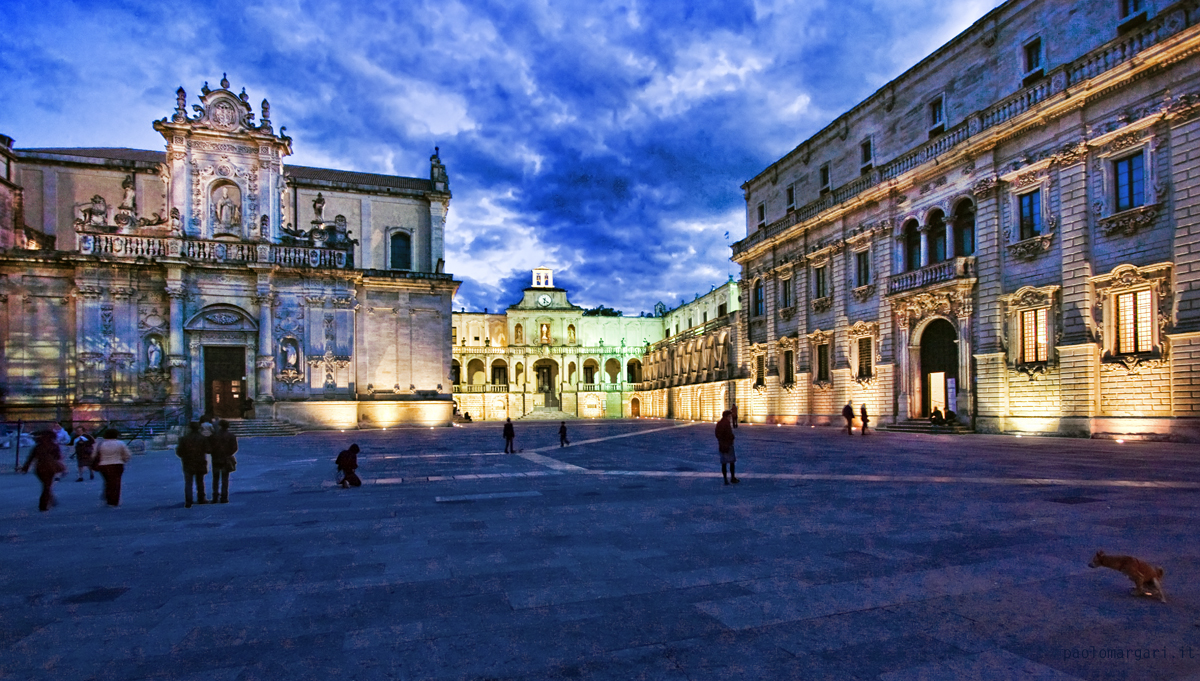
\includegraphics[height=1.05\paperheight]{Lecce1.jpg}};}
\begin{frame}
\centering
\footnotesize
\maketitle
\vspace{-.25cm}
\tiny{\textbf{Acknowledgements:} SeaDataNet, EMODnet Chemistry, \\
EMODnet Biology, STARESO}
\vspace{.125cm}

\begin{figure}
\centering

\includegraphics[width=.1\paperwidth]{gherlogo_transparent.PNG}\hspace*{.5cm}
\includegraphics[width=.1\paperwidth]{logo_ulg}\hspace*{.5cm}
\includegraphics[width=.1\paperwidth]{Logo_SeaDataNet_fond_transparent}\hspace*{.5cm}
\includegraphics[width=.07\paperwidth]{logo_emodnet}\hspace*{.5cm}
\includegraphics[width=.09\paperwidth]{Logo_Stareso}
\end{figure}

\end{frame}
}}
%-------------------------------------------------------------------------

\parindent 0cm

\author[Alexander Barth, Aida Alvera-Azc\'{a}rate, Mohamed~Ouberdous, Charles~Troupin, Sylvain~Watelet \& Jean-Marie~Beckers]{Alexander Barth, Aida Alvera-Azc\'{a}rate, Mohamed~Ouberdous,\\
 Charles~Troupin, Sylvain~Watelet \& Jean-Marie~Beckers}
  
\title[]{\diva workshop 2015}
\subtitle{\diva in 4 dimensions (GODIVA)}
\date{}
\begin{document}

\maketitlepage % defined in GHERheader2014.tex


%--------------------------------------------------------------------------------------------------------

\AtBeginSubsection[]
{
  \begin{frame}<beamer>{Outline}
    \tableofcontents[currentsection,currentsubsection]
  \end{frame}
}


\begin{frame}{Outline}
  \tableofcontents
  % You might wish to add the option [pausesections]
\end{frame}


\section{Getting Godiva and installation}
%-----------------------------------------


\begin{frame}[c]
\frametitle{Installation}
\huge
See Tutorial on installation \href{run:./DivaWorkshop2015_installation.pdf}{\important{(pdf)}}


\end{frame}


%%%%%%%%%%%%%%%%%%%%%%%%%%%%%%%%%%%%%%%%%%%%%%%%%%%%%%%%%%%%%%%%%
\subsection{Diva input info files}
%%%%%%%%%%%%%%%%%%%%%%%%%%%%%%%%%%%%%%%%%%%%%%%%%%%%%%%%%%%%%%%%%

\begin{frame}
\frametitle{\diva input info files}

\centerline{In \directory{input} directory:}

\begin{itemize}
\item {Edit} info files and adapt them to your case by providing in the relevant information
\end{itemize}


{\small
\begin{table}
\centering
\begin{tabular}{ll}
\toprule 
File name 					& content\\
\midrule 
\file{contour.depth} 		& list file of all depths in meters \\ 
\file{NCDFinfo} 			& metadata information for climatology NetCDF files \\ 
\file{general\_info} 		& information for metadata XML files generation \\ 
%{  NCDFNCDFinfo\_salinity} & metadata information for hydrostatic \\
%{  NCDFinfo\_temperature}  &  stabilisation procedure NetCDF files. \\
\bottomrule
\end{tabular}
\end{table}

}

\end{frame}

%%%%%%%%%%%%%%%%%%%%%%%%%%%%%%%%%%%%%%%%%%%%%%%%%%%%%%%%%%%%%%
\section{Data sets and domain grid preparation}
%%%%%%%%%%%%%%%%%%%%%%%%%%%%%%%%%%%%%%%%%%%%%%%%%%%%%%%%%%%%%%

%%%%%%%%%%%%%%%%%%%%%%%%%%%%%%%%%%%%%%%%%%%%%%%%%%%%%%%%%%%%%%
\subsection{Depths data sets extraction}
%%%%%%%%%%%%%%%%%%%%%%%%%%%%%%%%%%%%%%%%%%%%%%%%%%%%%%%%%%%%%%

\begin{frame}{Data extraction: input files preparation}

\centerline{In \directory{Climatology} directory:}

\begin{itemize}
%\item ODV4 spreadsheet(s) of your data
\item \file{datasource} file: list of paths to \important{ODV4 spreadsheet(s)} from which data sets will be extracted.
\item \file{varlist}, \file {yearlist} and \file {monthlist} files.
\item \file{qflist} (quality flags) file if desired.
\end{itemize}
\vspace{0.3cm}
\centerline{
\begin{tabular}{lcr}
\toprule
\file{varlist}& \file{yearlist} & \file{monthlist}\\
\midrule
Temperature   & 19002012 & 0101 \\
Salinity      &          & 0202 \\
              &          & 0303 \\
              \bottomrule
%\hline %& \hline& \hline
\end{tabular}
}

\end{frame}

%%%%%%%%%%%%%%%%%%%%%%%%%%%%%%%%%%%%%%%%%%%%%%%%%%%%%%%%%%%%%%

\begin{frame}
\frametitle{Data extraction: \file{driver} configuration \& \command{divadoall} }

%[containsverbatim]

\centerline{In \directory{Climatology} directory:}

\begin{itemize}
\item Edit the \file{driver} file and put in a flag number for data extraction.
\end{itemize}

\begin{figure}
\centering
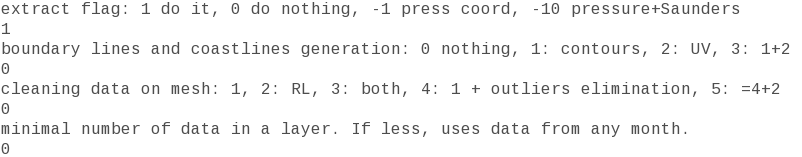
\includegraphics[width=8cm]{driverB}
\caption{\file{driver} file configuration example.}
\end{figure}

%\vspace{-0.3cm}

\begin{itemize}
\item Run \command{divadoall} or \command{godiva} (basic error check-up included)
\item Rem : do not forget to adapt the PATH (for ex. in \file{.bashrc})
\end{itemize}

A subdirectory \directory{divadata} is created in \directory{input} directory, and contains the data sets.

\end{frame}

%%%%%%%%%%%%%%%%%%%%%%%%%%%%%%%%%%%%%%%%%%%%%%%%%%%%%%%%%%%%%%
\subsection{Topography preparation \& Coastlines files generation}
%%%%%%%%%%%%%%%%%%%%%%%%%%%%%%%%%%%%%%%%%%%%%%%%%%%%%%%%%%%%%%

\begin{frame}[fragile]
\frametitle{Topography preparation: Diva-On-Web}

\url{http://gher-diva.phys.ulg.ac.be/web-vis/diva.html}

After creating this file :

\begin{verbatim}
lonmin latmin value
lonmax latmax value
\end{verbatim}

\begin{enumerate}
\item Upload the file on Diva-On-Web
\item Specify the output grid
\item Perform the analysis
\item Download the NetCDF file \file{diva\_bath.nc}
\item Put it in \directory{input}
\end{enumerate}

\begin{lstlisting}[style=Bash]
swatelet@gher ~/DIVA/diva-4.6.11/DIVA3D/divastripped/input $ ../../bin/divabath2topogrd.a
\end{lstlisting}

\end{frame}

%%%%%%%%%%%%%%%%%%%%%%%%%%%%%%%%%%%%%%%%%%%%%%%%%%%%%%%%%%%%%%

\begin{frame}[fragile]
\frametitle{Topography preparation: Diva-On-Web}

=> \file{topo.grd} and \file{TopoInfo.dat} are created \\
\vspace{5mm}
If you need to erase zones, just create a mask beforehand :

\begin{itemize}
\item Name : masktopo.nc
\item Axis : (LON and LAT) or (lon and lat)
\item Variable : MASKTOPO
\item Convention : 0 is erased, 1 is kept
\end{itemize}

\end{frame}

%%%%%%%%%%%%%%%%%%%%%%%%%%%%%%%%%%%%%%%%%%%%%%%%%%%%%%%%%%%%%%
\begin{frame}
\frametitle{Topography preparation, old method: \command{gebcomodif}}

\centerline{
 For a GEBCO topography file, use the script file \command{gebcomodif} to:
}
\small{
\begin{itemize}
\item Eliminate header lines
\item Change depth values from negative to positive values
\item Change comas to dots in decimal numbers 
\item Change longitude values from $[$0:360$]$ to $[$-180:180$]$ range
\item Mask rectangle regions by giving coordinates \\
in a \file{takeout.coord} file
\end{itemize}
}
\end{frame}

%%%%%%%%%%%%%%%%%%%%%%%%%%%%%%%%%%%%%%%%%%%%%%%%%%%%%%%%%%%%%%

\begin{frame}
\frametitle{Topography preparation}

\centerline{In \directory{input}:}
\begin{itemize}
\item \small Provide a topography file named \file{topogebco.asc} \\
 extracted from GEBCO Global Elevation Data.
\end{itemize}

\centerline{In the \directory{Climatology} directory:}

\begin{itemize}
\item \small Provide a \file{takeout.coord} file:
\end{itemize}

\vspace{-0.5cm}
\begin{table}
\tiny
\centering
\begin{tabular}{|cccc|}
\hline
Minlon1 & Maxlon1 & Minlat1 & Maxlat1\\
Minlon2 & Maxlon2 & Minlat2 & Maxlat2\\
Minlon3 & Maxlon3 & Minlat3 & Maxlat3\\
   .    &   .   &   .   &  .   \\
   .    &   .   &   .   &  .   \\
\hline
\end{tabular}
\end{table}

\vspace{-0.5cm}
\begin{itemize}
\item Run \file{gebcomodif} script file.
\end{itemize}
\Large{
\centerline{A \file{topo.gebco} file is generated in \directory{input}.}
}
\end{frame}

%%%%%%%%%%%%%%%%%%%%%%%%%%%%%%%%%%%%%%%%%%%%%%%%%%%%%%%%%%%%%%
\begin{frame}
\frametitle{Masking regions in topography}

\begin{figure}
\centering
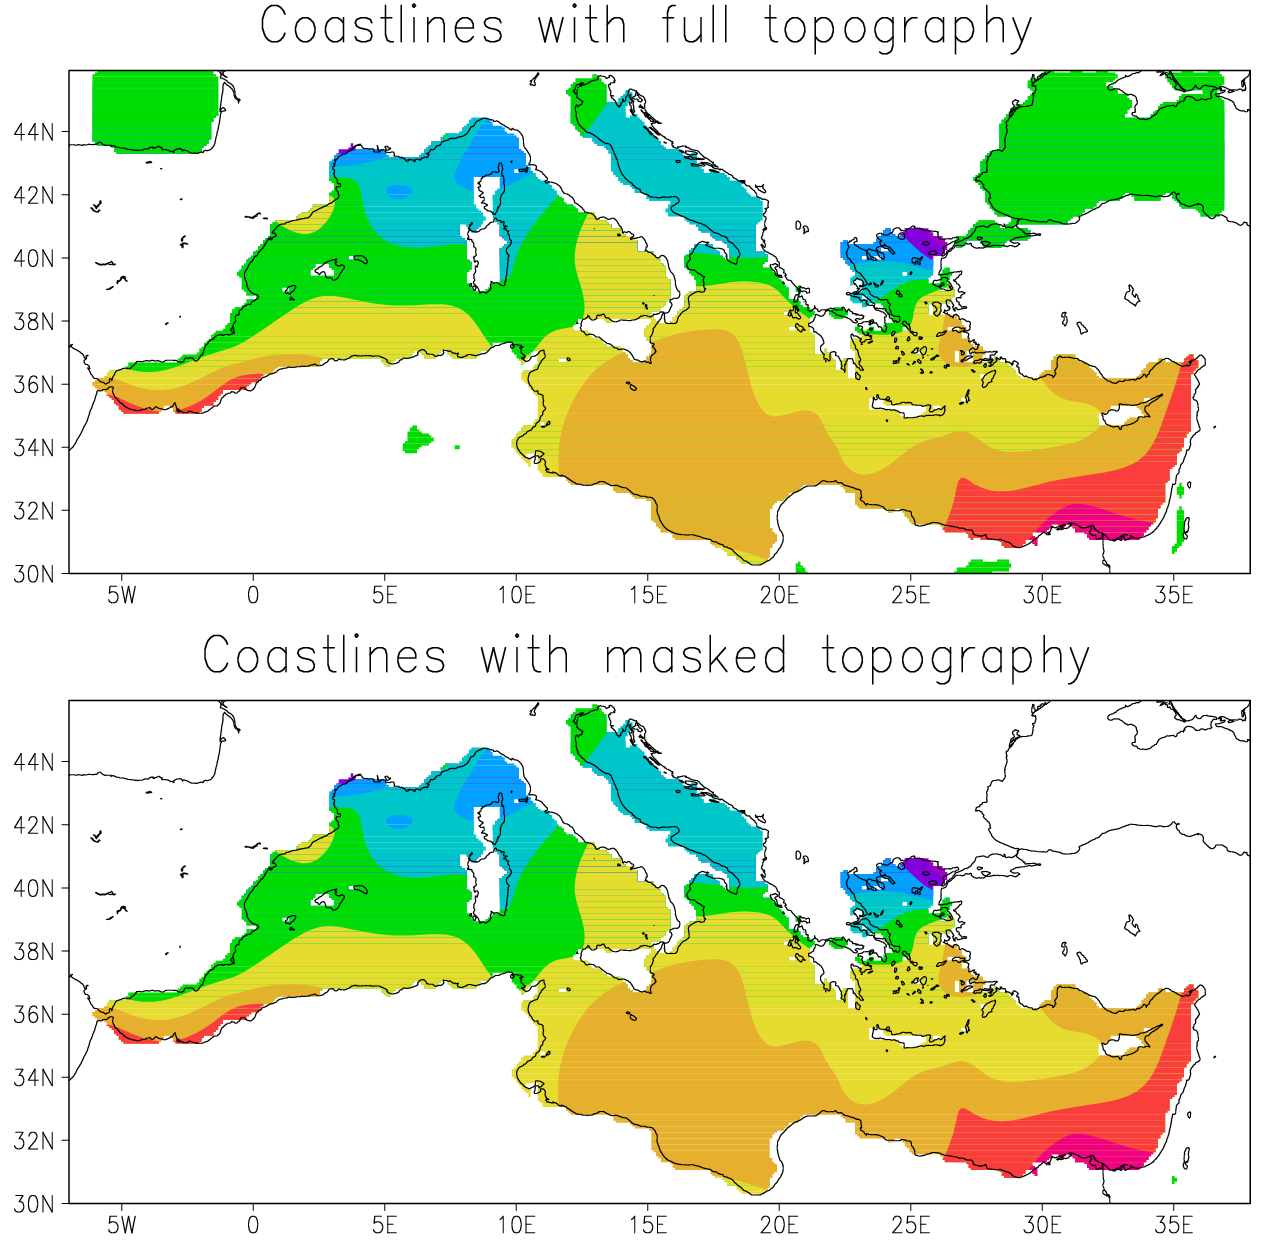
\includegraphics[width=.75\textwidth]{coastlines.png}
\end{figure}
\end{frame}

%%%%%%%%%%%%%%%%%%%%%%%%%%%%%%%%%%%%%%%%%%%%%%%%%%%%%%%%%%%%%%

\begin{frame}
\frametitle{Example of topography preparation}

\begin{itemize}
\item In \directory{input}, we provide \file{topogebco.asc} covering  the Mediterranean Sea area: 30$^{\circ}$N to 46$^{\circ}$N and 6$^{\circ}$W to 37$^{\circ}$E.
\item In \directory{Climatology}, we provide a \file{takeout.coord} file:
\end{itemize}

\begin{table}
\small
\centering
\begin{tabular}{|l|}
\hline
-6. -1. 42. 46.\\
26.5 40. 40. 46.\\
5. 9. 33. 35.\\
20. 30. 30. 30.5\\
35. 37. 31. 33.\\
\hline
\end{tabular}
\end{table}

After running the command \command{gebcomodif} in \directory{Climatology} directory, we obtain a \file{topo.gebco} in \directory{input} directory.

\begin{itemize}
\item \important{Or you can extract topography from diva-on-web !}
\end{itemize}

\end{frame}


%%%%%%%%%%%%%%%%%%%%%%%%%%%%%%%%%%%%%%%%%%%%%%%%%%%%%%%%%%%%%%

%%%%%%%%%%%%%%%%%%%%%%%%%%%%%%%%%%%%%%%%%%%%%%%%%%%%%%%%%%%%%%%%%

%\section{The {  driver} file: What \diva can do}

%\subsection{Coastlines files generation}

%%%%%%%%%%%%%%%%%%%%%%%%%%%%%%%%%%%%%%%%%%%%%%%%%%%%%%%%%%%%%%

\begin{frame}[t]
\frametitle{Coastline files generation: input files}

\centerline{In \directory{input} directory provide:}

\begin{columns}[totalwidth=\textwidth,T]
\column{.5\textwidth}
\vspace*{1cm}
\small{
\begin{itemize}
\item 
\begin{itemize}
\item[(a)] a \file{topo.gebco} file \hfill \important{OR}
\item[(b)] a \file{topo.dat} file \hfill \important{OR}
\item[(c)] \file{topo.grd} $+$ \file{TopoInfo.dat} files
\end{itemize}
\item the \file{contour.depth} file
\item a \file{param.par} file
\end{itemize}
}
\column{.5\textwidth}

\begin{figure}
\centering
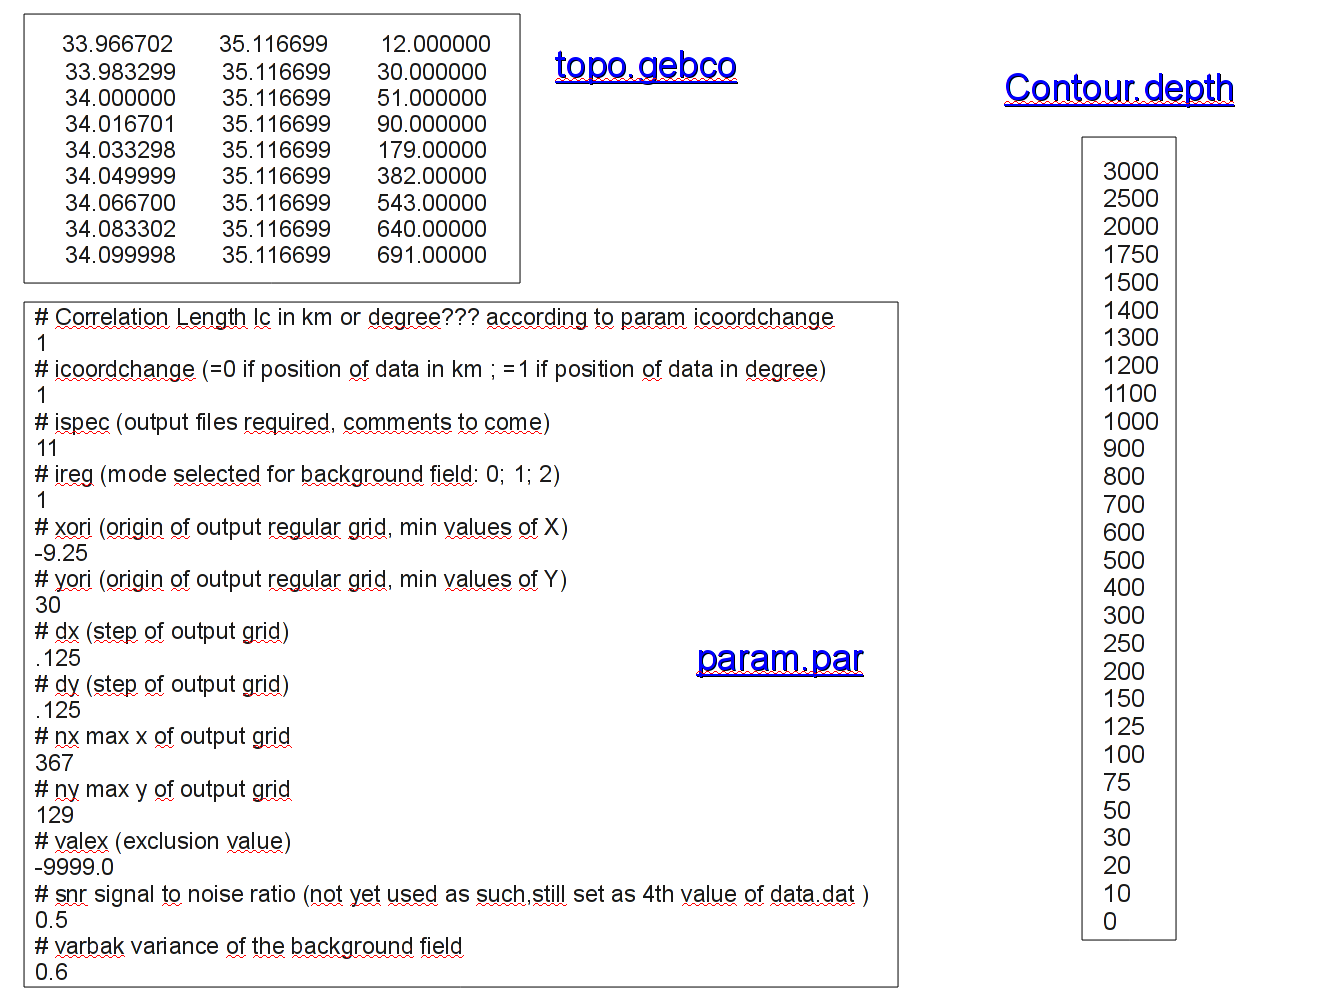
\includegraphics[width=6.5cm]{tocopa}
\end{figure}

\end{columns}
\end{frame}

%%%%%%%%%%%%%%%%%%%%%%%%%%%%%%%%%%%%%%%%%%%%%%%%%%%%%%%%%%%%%%

\begin{frame}
\frametitle{Coastlines files generation: \file{driver} configuration}

\centerline{In \directory{Climatology} directory:}
\small{
\begin{itemize}
\item Edit the \file{driver} file and choose a flag number\\
 for boundary lines and coastlines generation:
\end{itemize}
}
\vspace{-0.5cm}

\begin{table}
\caption{\file{driver} options for coastlines generation}

%\centerline{\shortstack{{  Driver options for coastlines} \\ {{}} \\ {{}}\\ {{}} \\ {{}}}}
\centering
\tiny
\begin{tabular}{|c|l|}
\hline 
{ { Comment line}}
 & 
\shortstack{ 
{ { Flag value and corresponding action}} }
\\ \hline  \hline  
 
\shortstack{ 
\\ \\
{Boundary lines and coastlines}\\
{ generation: } }
&
\begin{tabular}{r|l}
{\sf $0:\ $ } & {\sf no action is performed} \\ \hline
{\sf $1:\ $ } & {\sf generation of contour files of boundaries and coastlines } \\ \hline
{\sf $2:\ $ } & {\sf generation of advection UV files of velocities along coasts} \\ \hline
{\sf $3:\ $ } & {\sf generation of contour files and advection UV files}
\end{tabular} 
\\ \hline 
\end{tabular}



\end{table}


\vspace{-0.1cm}

\begin{figure}
\centering
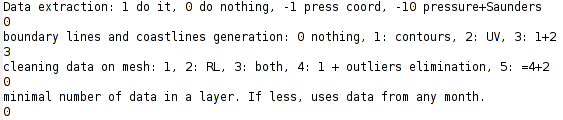
\includegraphics[width=8cm]{driver1}
\caption{\file{driver} file configuration example.}
\end{figure}

%\vspace{-0.3cm}
%\vspace{-0.1cm}
%\small{
%\begin{itemize}
%\item  {  run} \command{divadoall}}
%\end{itemize}
%}
\end{frame}

%%%%%%%%%%%%%%%%%%%%%%%%%%%%%%%%%%%%%%%%%%%%%%%%%%%%%%%%%%%%%%%%%

%%%%%%%%%%%%%%%%%%%%%%%%%%%%%%%%%%%%%%%%%%%%%%%%%%%%%%%%%%%%%%

\begin{frame}
\frametitle{Coastlines files generation: output}

\centerline{In \directory{Climatology} directory}

\begin{itemize}
\item Run \command{divadoall}
\end{itemize}
 
\vspace{0.5cm}

\centerline{
{A \directory{newinput} directory is created} which contains:
}
\begin{itemize}
\item \directory{divaparam}: a subdirectory where coastline files \file{coast.cont.100xx} are stored
\item \directory{divaUVcons\_all}: a subdirectory where velocity field files are stored
\end{itemize}

%\centerline{ {  TO DO:}}
\Large{
\begin{center}
Copy \directory{divaparam} and \directory{divaUVcons\_all} \\
to your \directory{input} directory.
\end{center}

}

\end{frame}

%%%%%%%%%%%%%%%%%%%%%%%%%%%%%%%%%%%%%%%%%%%%%%%%%%%%%%%%%%%%%%%%%
\subsection{Cleaning of data sets}
%%%%%%%%%%%%%%%%%%%%%%%%%%%%%%%%%%%%%%%%%%%%%%%%%%%%%%%%%%%%%%

\begin{frame}
\frametitle{Data Cleaning: input files}

\centerline{In \directory{input} directory:}

\begin{itemize}
\item \directory{divadata}: directory which contains data set files of the considered layers.
\item \directory{divaparam}: directory which contains coastline \file{coast.cont.100xx} files for all considered layers.
\item the \file{contour.depth} file.
\item a \file{param.par} file.
\end{itemize}

\end{frame}

%%%%%%%%%%%%%%%%%%%%%%%%%%%%%%%%%%%%%%%%%%%%%%%%%%%%%%%%%%%%%%

\begin{frame}
\frametitle{Data Cleaning: input files}

\centerline{In \directory{Climatology} directory}

\begin{itemize}
\item Provide \file{varlist}, \file{yearlist} and \file{monthlist} files.
\end{itemize}
\begin{itemize}
\item Edit the \file{driver} file,
\item Choose a flag number for data cleaning and
\item give the considered minimum layer and maximum layer numbers.
\end{itemize}

\end{frame}

%-----------------------------------------------------------------------------------------------------

\begin{frame}
\frametitle{Data Cleaning: driver configuration}

\begin{table}
\centering
\caption{\file{driver} options for data cleaning}
\tiny{
\begin{tabular}{|c|l|}
\hline 
{ { Comment line}}
 & 
\shortstack{ 
{ { Flag value and corresponding action}} }
\\ \hline  \hline  
 
\shortstack{ 
\\ \\
{cleaning data on mesh}\\
{ } }
&
\begin{tabular}{r|l}
{\sf $0:\ $ } & {\sf no action is performed} \\ \hline
{\sf $1:\ $ } & {\sf cleaning data out of the mesh} \\ \hline
{\sf $2:\ $ } & {\sf generation of relative length (RL) fields} \\ \hline
{\sf $3:\ $ } & {\sf cleaning data out of the mesh and generations of RL fields} \\ \hline
{\sf $4:\ $ } & {\sf cleaning data set files from outliers} \\ \hline
{\sf $5:\ $} & {\sf  generations of RL fields and cleaning data set files from outliers}
\end{tabular} 
\\ \hline 
\end{tabular}
}\end{table}

\vspace{-0.3cm}

\begin{figure}
\centering
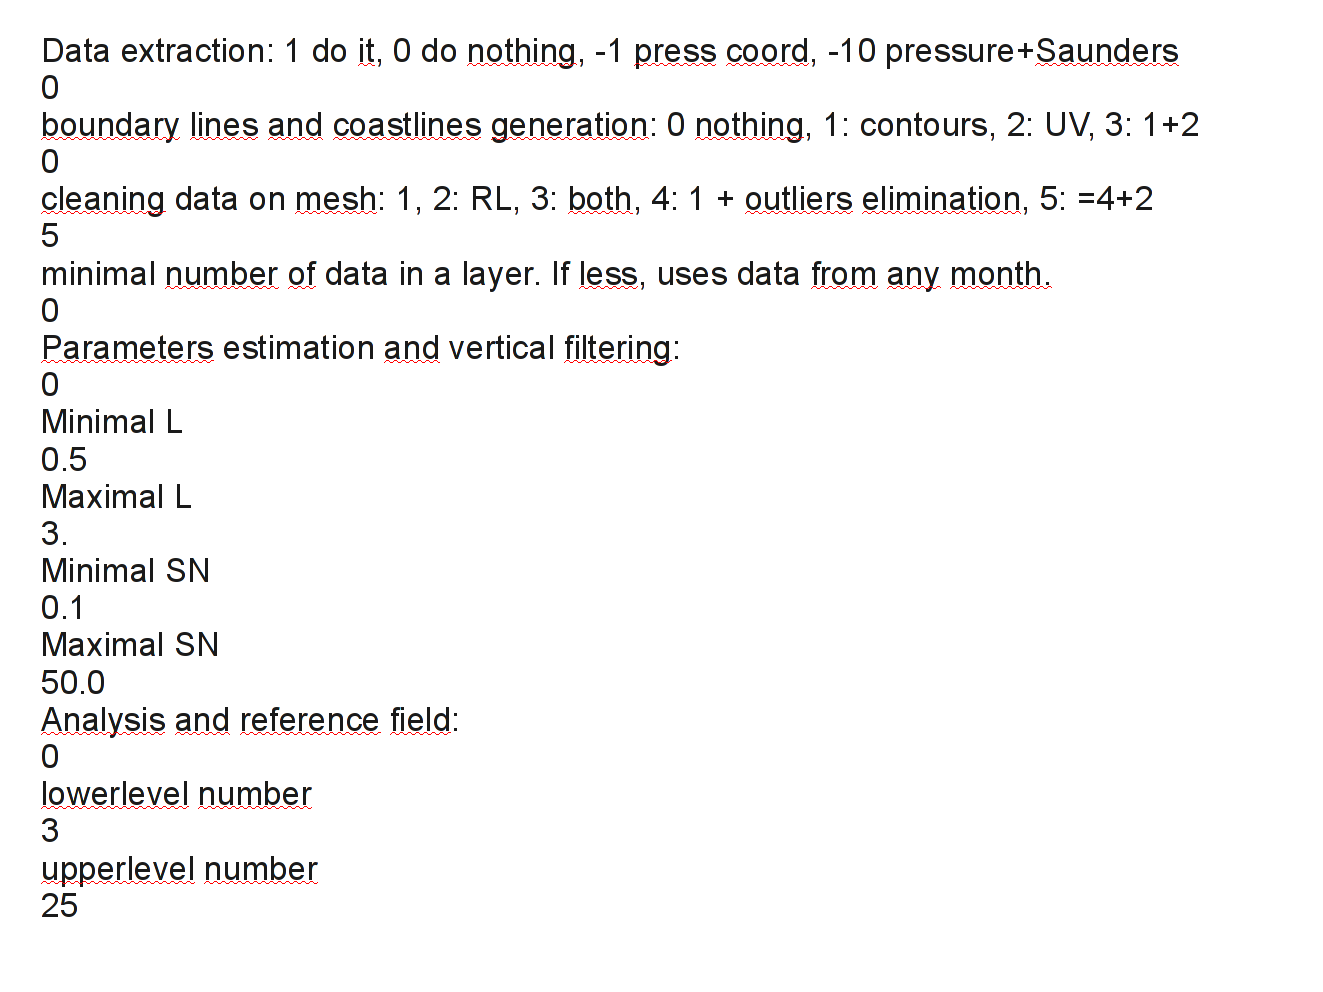
\includegraphics[width=6cm]{driver3}
\caption{\file{driver} file configuration example.}
\end{figure}
\end{frame}

%---------------------------------------------------------------------------------------

\begin{frame}
\frametitle{Data Cleaning: output}

\centerline{In \directory{Climatology} directory:}
\vspace{0.5cm}

{Run \command{divadoall}}.


A \directory{newinput} directory is created and contains:
\begin{itemize}
\item \directory{divadata} subdirectory which contains cleaned data sets
\item \directory{divadata} subdirectory which contains relative length files if generated
\end{itemize}

\Large{
\begin{center}
Copy the content of\\ 
\directory{newinput/divadata} and \directory{newinput/divaparam} \\
to \directory{input/divadata} and \directory{input/divaparam} directories.
\end{center}
}


\end{frame}

%%%%%%%%%%%%%%%%%%%%%%%%%%%%%%%%%%%%%%%%%%%%%%%%%%%%%%%%%%%%%%%%%
\subsection{Optimisation of $L$ and $\snr$ parameters}
%%%%%%%%%%%%%%%%%%%%%%%%%%%%%%%%%%%%%%%%%%%%%%%%%%%%%%%%%%%%%%

\begin{frame}
\frametitle{Parameters optimisation: input}

\centerline{In \directory{input} directory provide:}
\begin{itemize}
\item \directory{divadata} directory which contains the data set files of the considered depths.
\item \directory{divaparam} directory which contains coastline \file{coast.cont.100xx} files of the considered basin.
\item The \file{contour.depth} file.
\item A (template) \file{param.par} file.
\end{itemize}

\end{frame}

%%%%%%%%%%%%%%%%%%%%%%%%%%%%%%%%%%%%%%%%%%%%%%%%%%%%%%%%%%%%%%

\begin{frame}
\frametitle{Parameters optimisation: input files}

\centerline{In \directory{Climatology} directory:}
\small{
\begin{itemize}
\item Provide \file{varlist}, \file{yearlist} and \file{monthlist} files
\item Edit the \file{driver} file and give a flag number for parameters optimisation and bounds for correlation length ($L$) and signal-to-noise ($\snr$) parameters.
\end{itemize}
}
\vspace{-0.3cm}

\begin{figure}
\centering
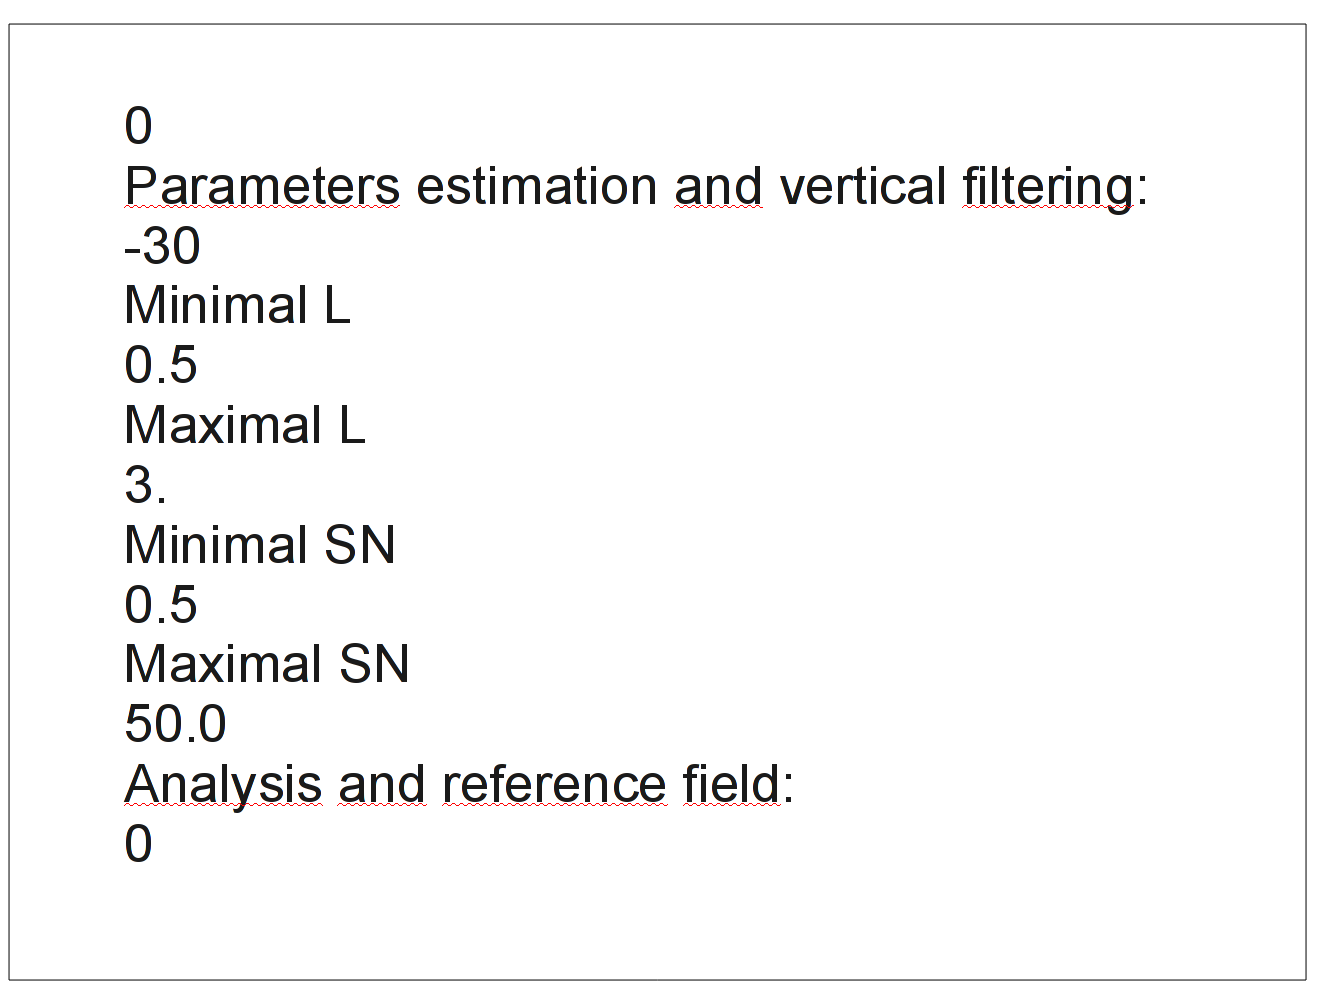
\includegraphics[width=5.5cm]{driver4}
\caption{\file{driver} file configuration example.}
\end{figure}

\end{frame}
%%%%%%%%%%%%%%%%%%%%%%%%%%%%%%%%%%%%%%%%%%%%%%%%%%%%%%%%%%%%%%

\begin{frame}
\frametitle{Parameters optimisation: \file{driver} configuration}

\begin{table}
%\centerline{\shortstack{{  Driver options for coastlines} \\ {{}} \\ {{}}\\ {{}} \\ {{}}}}
\centering
\caption{\file{driver} options for parameters optimisation.}
\tiny{
\begin{tabular}{|c|l|}
\hline  
{ { Comment line}}
 & 
\shortstack{ 
{ { Flag value and corresponding action}} }
\\ \hline  \hline  
 
\shortstack{ 
\\ \\
{Parameters optimisation}\\
{and vertical filtering } }
&
\begin{tabular}{r|l}
{\sf $0\ \ :\ $} & {\sf  no action is performed} \\ \hline
{\sf $1\ \ :\ $} & {\sf  estimation for each level of correlation length $L$ parameter} \\ \hline
{\sf $2\ \ :\ $} & {\sf  estimation for each level of signal to noise ratio ($\snr$) parameter} \\ \hline
{\sf $-1\ :\ $} & {\sf  estimation and vertical filtering of $L$ parameter} \\ \hline
{\sf $-2\ :\ $} & {\sf  estimation and vertical filtering of $\snr$ parameter } \\ \hline
{\sf $3\ \ :\ $} & {\sf  estimation for each level of $L$ and $\snr$ parameters} \\ \hline
{\sf $-3\ :\ $} & {\sf  estimation and vertical filtering of $L$ and $\snr$ parameters} \\ \hline
{\sf $10\ :\ $} & {\sf  estimation of $L$ parameter for each level using data mean distance} \\
& {\sf as a minimum} \\ \hline
{\sf $-10:\ $} & {\sf  estimation of $L$ parameter using data mean distance as a minimum} \\
& {\sf and vertical filtering} \\ \hline
{\sf $30\ :\ $} & {\sf  estimation of $\snr$ and $L$ parameters for each level, using data} \\
& {\sf mean distance as a minimum for $L$} \\ \hline
{\sf $-30:\ $} & {\sf  estimation and vertical filtering of $\snr$ and $L$ parameters,} \\
& {\sf  using data mean distance as a minimum for $L$,} 
\end{tabular} 
\\ \hline 
\end{tabular}
}
\end{table}

\end{frame}

%%%%%%%%%%%%%%%%%%%%%%%%%%%%%%%%%%%%%%%%%%%%%%%%%%%%%%%%%%%%%%

\begin{frame}
\frametitle{Parameters optimisation: output}

\centerline{In \directory{Climatology} directory:}
%\vspace{-0.5cm}

\begin{itemize}
\item Run the \command{divadoall} script file.
\end{itemize}

{A \directory{newinput} directory is created and contains:}

\begin{itemize}
\item[ ] \directory{divaparam} subdirectory with \file{param.par.100xx} files and summary files of the optimisation and filtering procedure.
\end{itemize}

\vfill 
\Large{
\begin{center}
Copy the  content of \directory{newinput/divaparam}\\
 to \directory{input/divaparam} directory
\end{center}
}

\end{frame}

%%%%%%%%%%%%%%%%%%%%%%%%%%%%%%%%%%%%%%%%%%%%%%%%%%%%%%%%%%%%%%%%%
\section{Producing a climatology}
\subsection{The analysis}
%%%%%%%%%%%%%%%%%%%%%%%%%%%%%%%%%%%%%%%%%%%%%%%%%%%%%%%%%%%%%%

\begin{frame}
\frametitle{Producing a Climatology: input}

\centerline{In \directory{input} directory:}

\begin{itemize}
\item \directory{divadata} directory which contains data sets for the considered layers,
\item \directory{divaparam} directory which contains:
\begin{itemize}
\item[] coastlines \file{coast.cont.100xx} files,
\item[] coastlines \file{param.par.100XX} files.
\end{itemize}
\item the \file{contour.depth} file, 
\item a \file{param.par} file if not provided in \directory{divaparam}
\end{itemize}

\end{frame}


%%%%%%%%%%%%%%%%%%%%%%%%%%%%%%%%%%%%%%%%%%%%%%%%%%%%%%%%%%%%%%

\begin{frame}
\frametitle{Producing a Climatology: input \& and driver}

\centerline{In \directory{Climatology} directory:}

\small{
\begin{itemize}
\item Provide
\begin{itemize}
\item[] \file{varlist},
\item[] \file{yearlist} and
\item[] \file{monthlist} files.
\end{itemize}
\item Edit the \file{driver} file and choose a flag number for analysis.
\end{itemize}
}

\begin{figure}
\centering
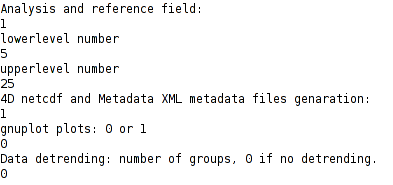
\includegraphics[width=5.5cm]{driver5}
\caption{\file{driver} file configuration example.}
\end{figure}

\end{frame}
%%%%%%%%%%%%%%%%%%%%%%%%%%%%%%%%%%%%%%%%%%%%%%%%%%%%%%%%%%%%%%

\begin{frame}
\frametitle{Producing a Climatology: input \& and driver}

\centerline{In \directory{Climatology} directory:}
%===========================================================
\begin{table}
%\centerline{\shortstack{{  Driver options for coastlines} \\ {{} \\ {{}}\\ {{}} \\ {{}}}}
\centering
\caption{\file{driver} options analyses \& climatologies production.}
\tiny{
\begin{tabular}{|c|l|}
\hline  
{ { Comment line}}
 & 
\shortstack{ 
{ { Flag value and corresponding action}} }
\\ \hline  \hline  
 
\shortstack{ 
\\ \\
{Analysis} \\
{and reference fields } }
&
\begin{tabular}{r|l}
{\sf $\ 0:\ $} & {\sf  no action is performed} \\ \hline
{\sf $\ 1:\ $} & {\sf  Perform analyses defined by a set of input files:  {  varlist}, {  yearlist},} \\
& {\sf \file{monthlist}, \file{constandrefe} and the files in \directory{input/} directory } \\ \hline
{\sf $\ 2:\ $} & {\sf  generation of reference field} \\ \hline
{\sf $\ 3:\ $} & {\sf  perform analyses as in $1$ based on vertically filtered background} \\ \hline
{\sf $11:\ $} & {\sf  perform analyses using a  $\log$(data)-$\exp$(analysis) transformations} \\ \hline
{\sf $13:\ $} & {\sf  perform analyses using the anamorphosis transformation} \\ \hline
{\sf $14:\ $} & {\sf  perform analyses using a user defined transformation} \\ \hline
{\sf $21:\ $} & {\sf  perform reference fields using a  $\log$(data)-$\exp$(analysis) transformations} \\ \hline
{\sf $23:\ $} & {\sf  perform reference fields using the anamorphosis transformation} \\ \hline
{\sf $24:\ $} & {\sf  perform reference fields using user defined transformation} \\ \hline
\end{tabular} \\
 & \\
 & {\sf \underline{{  Adding $100$}} to flag values $1$, $11$, $13$ and $14$ allows to perform}\\
 & {\sf the same action using a reference field for each layer generated on the basis of}\\
 & {\sf all data from the two neighbouring layers in addition to the layer data set.}\\ 
 & \\
 & {\sf \underline{{  Adding $100$}} to flag values $2$, $21$, $23$ and $24$ allows to perform } \\
& {\sf reference fields with the same action using all data from the two neighbouring }\\
 & {\sf layers in addition to the layer data set}\\ \hline
%\\ \hline 
\end{tabular}
}
\end{table}

\vfill 

Run \command{divadoall} script file.

\end{frame}
%%%%%%%%%%%%%%%%%%%%%%%%%%%%%%%%%%%%%%%%%%%%%%%%%%%%%%%%%%%%%%%%%

\begin{frame}
\frametitle{Producing a Climatology: output}

\centerline{An \directory{output/3Danalysis} directory}
\centerline{is created and contains:}

\begin{itemize}
\item The 4D climatology NetCDF file:
\begin{itemize}
\item[] {\Large \resfile{Temperature.19002010.4Danl.nc}}
\end{itemize}
\end{itemize}

\begin{itemize}
\item subdirectories:\par
 \directory{Fields}: contains all \diva\ analyses 2D-fields\par
 \directory{Meshes}: contains depths meshes for each layer
\item 3D NetCDF and  binary (GHER format) files:\par
{\scriptsize
 \resfile{Temperature.19002010.nnmm.100xx.100yy.anl.nc} \par
 \resfile{Temperature.19002010.nnmm.100xx.100yy.fieldgher.anl}
 }
 \item \important{+ 4D netcdf files (\resfile{Temperature.4Danl.nc}) if netcdf flag = 11 or -11 !}
\end{itemize}

\end{frame}

%%%%%%%%%%%%%%%%%%%%%%%%%%%%%%%%%%%%%%%%%%%%%%%%%%%%%%%%%%%%%%%%%
\subsection{Using advection fields}

%%%%%%%%%%%%%%%%%%%%%%%%%%%%%%%%%%%%%%%%%%%%%%%%%%%%%%%%%%%%%%%%%

\begin{frame}
\frametitle{Production of a Climatology using advection fields} 

\centerline{In \directory{input} directory provide:}
\begin{itemize}
\item \directory{divadata} directory (data sets)
\item \directory{divaparam} directory \par (\file{coast.cont.100xx} and \file{param.par.100xx} files)
\item \directory{divaUVcons\_all} directory which contains velocity fields:\par (GHER-format) binary files. (+ see \command{asctobin})
\item the \file{contour.depth}
\item a \file{param.par} if not provided in \directory{divaparam}
\end{itemize}

\centerline{In \directory{input/divaUVcons\_all} provide}
\begin{itemize}
\item \file{constraint.dat} (one line) file.
\end{itemize}
\centerline{
\begin{tabular}{|l|}\hline
10 \quad 0\\
\hline
\end{tabular}
}
%\vspace{-0.3cm}
{\tiny \centerline{example: \file{constraint.dat} file} }

\end{frame}

%%%%%%%%%%%%%%%%%%%%%%%%%%%%%%%%%%%%%%%%%%%%%%%%%%%%%%%%%%%%%%%%%

\begin{frame}
\frametitle{Production of a Climatology using advection fields} 

\centerline{In \directory{Climatology} directory:}

\begin{itemize}
\item provide a \file{constandrefe} file:
\begin{table}
\centering
\caption{Example of \file{constandrefe} file.}

\small{
\begin{tabular}{|l|}
\hline
\# advection flag\\
1\\
\# reference field flag\\
0\\
\# variable year code \\
00000000\\
\# variable month code\\
0000\\
\hline
\end{tabular}
}
\end{table}
%\begin{itemize}
\item Provide \file{varlist}, \file{yearlist} and \file{monthlist} files.
\item Edit the \file{driver} file and choose a flag number for analysis.
\item Execute \command{divadoall}.
\end{itemize}


\end{frame}
%%%%%%%%%%%%%%%%%%%%%%%%%%%%%%%%%%%%%%%%%%%%%%%%%%%%%%%%%%%%%%
\subsection{Using reference fields}
%\subsubsection{Data extraction for reference fields}

%%%%%%%%%%%%%%%%%%%%%%%%%%%%%%%%%%%%%%%%%%%%%%%%%%%%%%%%%%%%%%

\begin{frame}
\frametitle{Data extraction for reference field}

\centerline{In \directory{input} directory:}
\begin{itemize}
\item the \file{contour.depth} file
\end{itemize}
\centerline{In \directory{Climatology} directory provide:}
\begin{itemize}
\item \file{datasource} file (ODV4 spreadsheet(s) path)
\item \file{varlist}, \file{yearlist} and \file{monthlist} files\par

\begin{tabular}{|l|c|r|}\hline
\toprule
\file{varlist}& \file{yearlist} & \file{monthlist}\\
\midrule
Temperature   & 19002010 & 0103 \\
\bottomrule
\end{tabular}
\item \file{qflist} file if desired
\item Edit the \file{driver} file and choose a flag number for data extraction
%\end{itemize}
%\vspace{0.1cm}
\item Run \command{divadoall} script file.
\end{itemize}

The variable(s) data set files are stored in  \directory{input/divadata} directory

\end{frame}


%%%%%%%%%%%%%%%%%%%%%%%%%%%%%%%%%%%%%%%%%%%%%%%%%%%%%%%%%%%%%%
%\subsubsection{Producing reference fields}
%%%%%%%%%%%%%%%%%%%%%%%%%%%%%%%%%%%%%%%%%%%%%%%%%%%%%%%%%%%%%%%%%

\begin{frame}
\frametitle{Production reference fields: inputs}

\centerline{In \directory{input} directory:}
\begin{itemize}
\item \directory{divadata} directory (data sets)
\item \directory{divaparam} directory \par (\file{coast.cont.100xx} and \file{param.par.100xx} files)
\item the \file{contour.depth}
\item a \file{param.par} if not provided in \directory{divaparam} with value equal to zero for ireg (ireg$=0$)
\end{itemize}

\centerline{In \directory{Climatology} directory:}
\begin{itemize}
\item Provide \file{varlist}, \file{yearlist} and \file{monthlist} files.
\item Edit the \file{driver} and choose flag value $1$ for data cleaning.
\item and flag value $2$, $21$, $23$ or $24$ for analysis.
\item Run \command{divadoall} script file.
\end{itemize}

\end{frame}


%%%%%%%%%%%%%%%%%%%%%%%%%%%%%%%%%%%%%%%%%%%%%%%%%%%%%%%%%%%%%%%%%

\begin{frame}
\frametitle{Production reference fields: output}

\centerline{\Large{A \directory{newinput} directory is created and contains:}}
\small{
\begin{itemize}
\item \directory{divarefe} subdirectory which contains reference fields (\diva 2D binary files) in GHER-format.
\end{itemize}
}

\centerline{\Large{In \directory{output/3Danalysis} directory:}}


\small{
\begin{itemize}
\item \directory{Fields}: contains all \diva analyses 2D-fields.
\item 3D NetCDF files:\par \resfile{Temperature.19002010.0103.100xx.100yy.ref.nc}
\item Binary 3D files (GHER-format):\par \resfile{Temperature.19002010.0103.100xx.100yy.fieldgher.ref}
\end{itemize}
}

%\vspace{0.5cm}

\centerline{\Large{Copy the content of \directory{newinput/divarefe} to}}

\centerline{\Large{\directory{input/divarefe\_all}}}

\end{frame}


%%%%%%%%%%%%%%%%%%%%%%%%%%%%%%%%%%%%%%%%%%%%%%%%%%%%%%%%%%%%%%
%\subsubsection{Producing Climatology using reference fields}

%%%%%%%%%%%%%%%%%%%%%%%%%%%%%%%%%%%%%%%%%%%%%%%%%%%%%%%%%%%%%%%%%

\begin{frame}
\frametitle{Producing Climatology using reference fields}

\centerline{In \directory{input} directory:}
\begin{itemize}
\item \directory{divadata} directory (data sets)
\item \directory{divaparam} (\file{coast.cont.100xx} and \file{param.par.100xx})
\item \directory{divarefe\_all} directory which contains reference fields
\item the \file{contour.depth} file.
\end{itemize}

\centerline{In \directory{Climatology} directory:}

\begin{itemize}
\item \file{constandrefe} file:
\small{
\begin{tabular}{|l|}
\hline
\# advection flag\\
0\\
\# reference field flag\\
1\\
\# variable year code \\
19002010\\
\# variable month code\\
0103\\
\hline
\end{tabular}
}
\end{itemize}
\end{frame}

%%%%%%%%%%%%%%%%%%%%%%%%%%%%%%%%%%%%%%%%%%%%%%%%%%%%%%%%%%%%%%%%%

\begin{frame}
\frametitle{Using reference fields}

\centerline{In \directory{Climatology} directory:}

\begin{itemize}
\item \file{varlist}, \file{yearlist} and \file{monthlist} files
%\begin{tabular}{|l|c|r|}\hline
%{  varlist}& {  yearlist} & {  monthlist}\\
%\hline
%Temperature   & 19002010 & 0101 \\
%              &          & 0202 \\
%              &          & 0303 \\
%\hline %& \hline& \hline
%\end{tabular}
\item Edit \file{driver} file and choose a flag number for analysis.
\item Run \command{divadoall} script file.
\end{itemize}

\vfill

Results will be stored in \directory{output/3Danalysis} directory.


\end{frame}

%%%%%%%%%%%%%%%%%%%%%%%%%%%%%%%%%%%%%%%%%%%%%%%%%%%%%%%%%%%%%%
\subsection{Detrending}

%%%%%%%%%%%%%%%%%%%%%%%%%%%%%%%%%%%%%%%%%%%%%%%%%%%%%%%%%%%%%%%%%

\begin{frame}
\frametitle{Detrending}


\centerline{In \directory{input} directory provide:}
\begin{itemize}
\item \directory{divadata} directory where data set files have more than five columns (5th, 6th, \ldots contain the information in which class the data point belongs)
\item same other inputs as for normal run
\end{itemize}

\centerline{In \directory{Climatology} directory}
\centerline{ provide the usual input text files and:}

\begin{itemize}
\item Edit the \file{driver} file and
\item choose a flag number for detrending a value (less or equal to the number of groups) present in your data set
\end{itemize}

\centerline{Run \command{divadoall} script file.}


\begin{itemize}
\item Results will be stored in
\end{itemize}
\centerline{ \Large \directory{output/3Danalysis} directory}.

\end{frame}


%--------------------------------------------------------------------------------------------------------

\begin{frame}[t]
\frametitle{To go further\ldots}

\vspace{.2cm}
\begin{columns}[totalwidth=1.1\textwidth,t]
\column{.65\textwidth}
\vspace{1cm}
\begin{overlayarea}{\textwidth}{5cm}
\begin{itemize}
\item<1-> Result layers are \textit{stacked} together

\item<2-> Problems may occur between two levels\ldots

\item<3-> \ldots so stabilisation is required

\end{itemize}
\end{overlayarea}

\column{.45\textwidth}
\begin{figure}
\centering
\includegraphics<1>[width=.7\columnwidth]{DSCN1615}
%\includegraphics<2>[width=.8\columnwidth]{}
\includegraphics<3>[width=.8\columnwidth]{Italia08_025}
\end{figure}

\end{columns}

\end{frame}

% -------------------------------------------------------------------------------------------------------------------------------------
\end{document}
